\documentclass[letterpaper,12pt]{article}
\usepackage[margin=.65in,top=.72in,bottom=.62in,headheight=16pt,headsep=15pt,footskip=19pt]{geometry}
\usepackage[T1]{fontenc}
\usepackage{lmodern,tikz,fancyhdr}\pdfmapfile{+lm.map}
\usetikzlibrary{arrows.meta,shapes.geometric}
\pagestyle{fancy}\fancyhf{}\renewcommand{\headrulewidth}{0pt}\renewcommand{\footrulewidth}{0pt}
\setlength{\parindent}{0pt}\setlength{\parskip}{0pt}
\fancyhead[L]{\small Week 46 / Two boards forget their starts / Grades 2--3}
\fancyfoot[L]{\footnotesize Bellingham Math Circle / Week 46 / W46-grades-2-3-v2}\fancyfoot[R]{\footnotesize\thepage}
\begin{document}
\noindent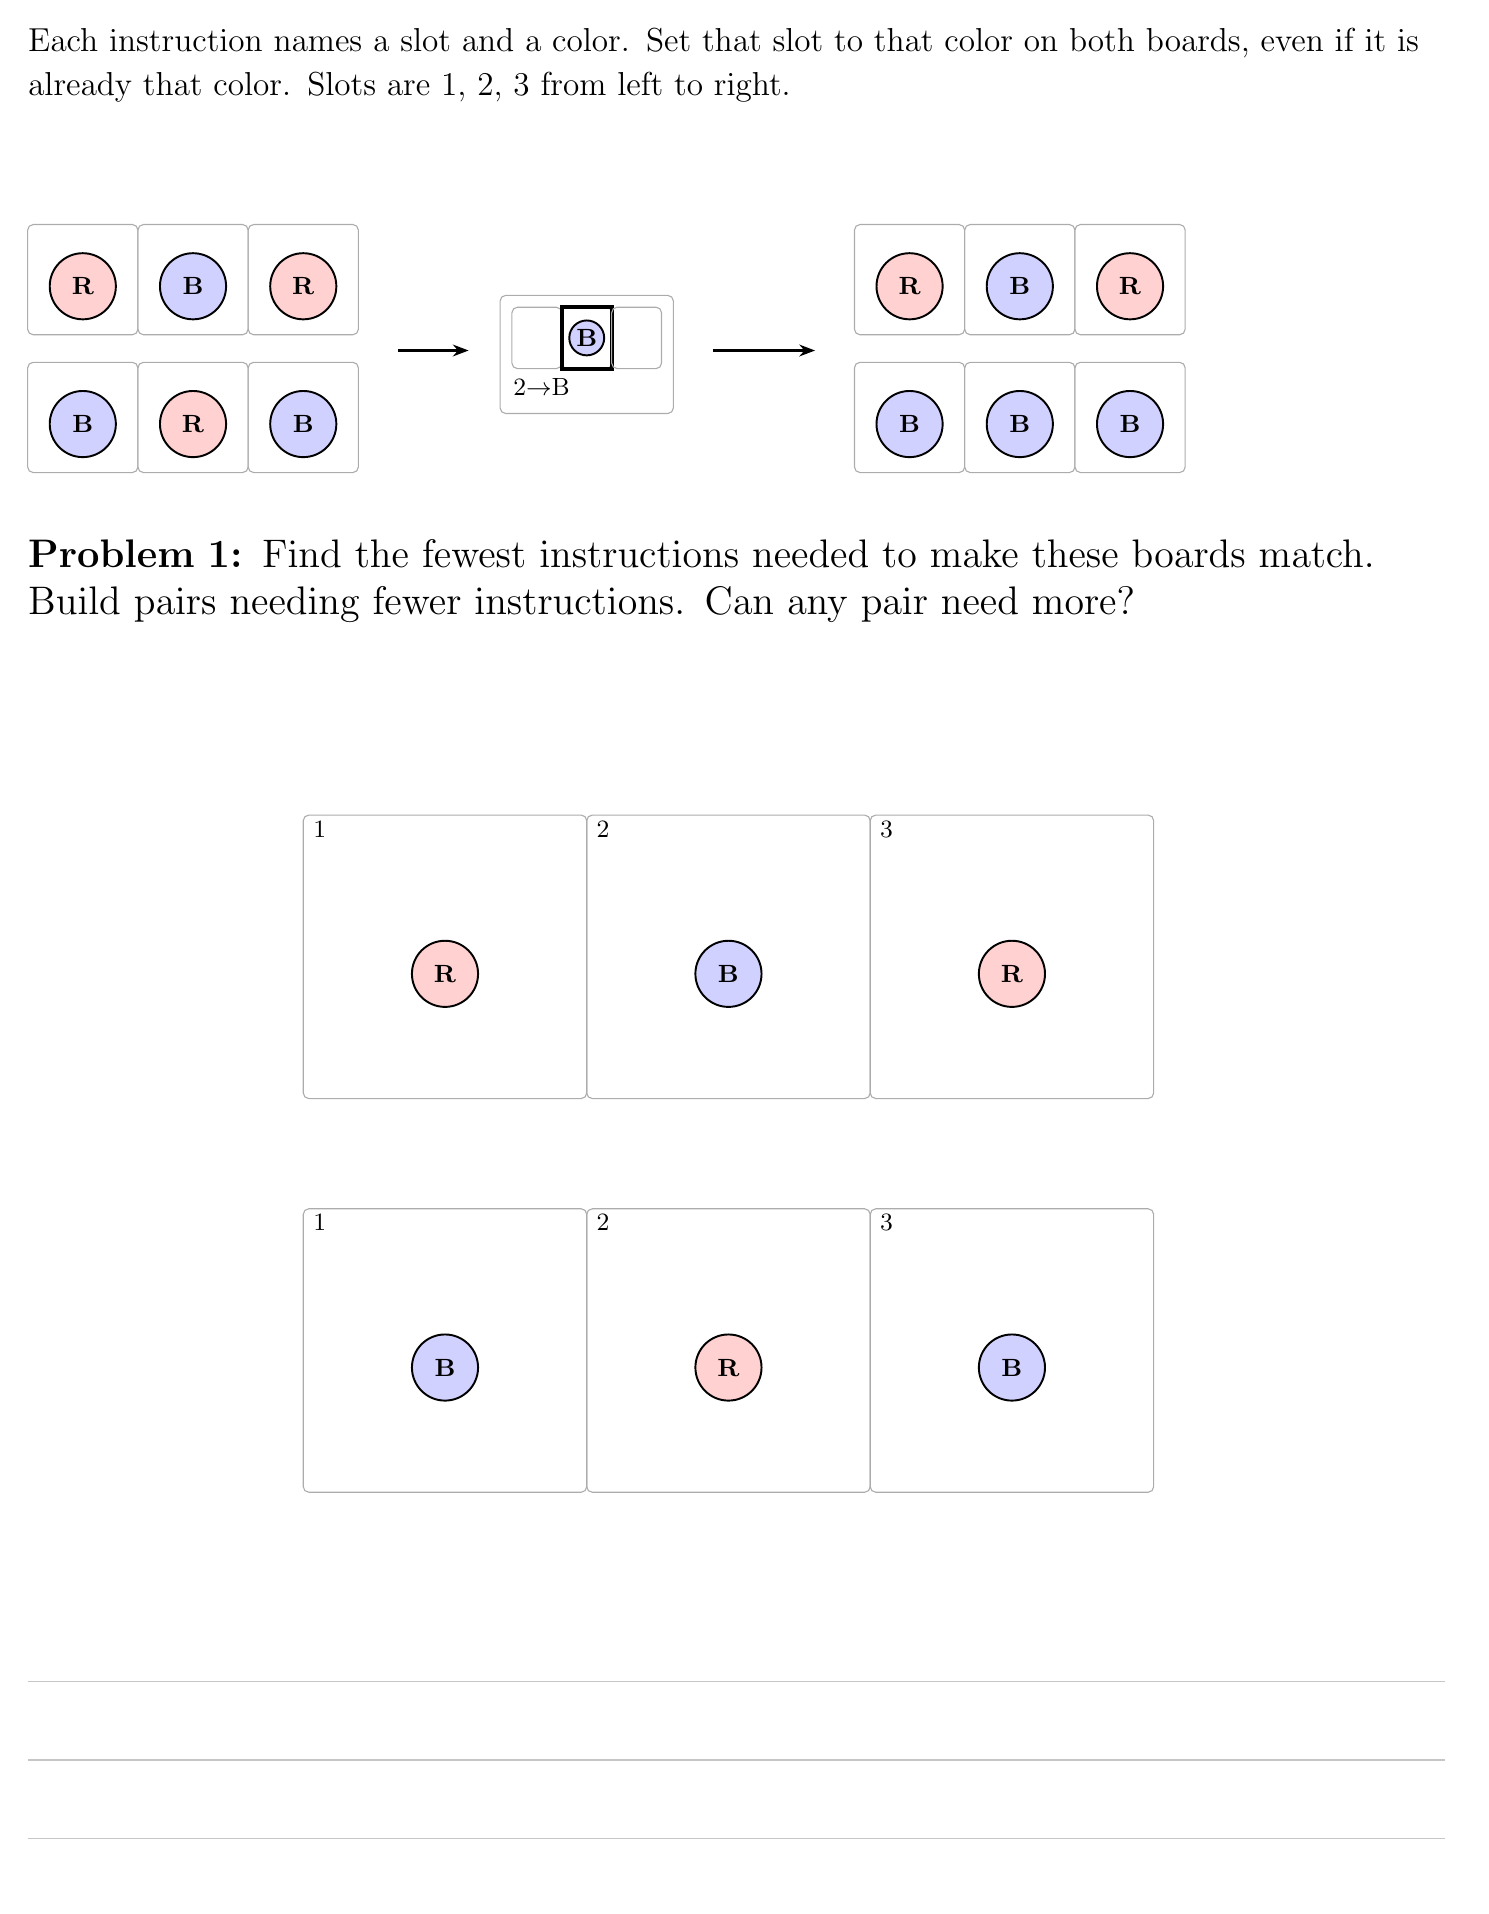
\begin{tikzpicture}[x=1cm,y=1cm]\path[use as bounding box] (0,0) rectangle (18.2,-23.6);
\node[anchor=north west,text width=18cm,inner sep=0pt,font=\fontsize{13}{16}\selectfont] at (0,0) {Each instruction names a slot and a color. Set that slot to that color on both boards, even if it is already that color. Slots are 1, 2, 3 from left to right.};
\draw[gray!65,rounded corners=2pt] (0.0,-2.5) rectangle (1.4,-3.9);
\draw[fill=red!18,line width=.7pt] (0.7,-3.284) circle (0.42);
\node[font=\bfseries\small] at (0.7,-3.284) {R};
\draw[gray!65,rounded corners=2pt] (1.4,-2.5) rectangle (2.8,-3.9);
\draw[fill=blue!18,line width=.7pt] (2.0999999999999996,-3.284) circle (0.42);
\node[font=\bfseries\small] at (2.0999999999999996,-3.284) {B};
\draw[gray!65,rounded corners=2pt] (2.8,-2.5) rectangle (4.199999999999999,-3.9);
\draw[fill=red!18,line width=.7pt] (3.5,-3.284) circle (0.42);
\node[font=\bfseries\small] at (3.5,-3.284) {R};
\draw[gray!65,rounded corners=2pt] (0.0,-4.25) rectangle (1.4,-5.65);
\draw[fill=blue!18,line width=.7pt] (0.7,-5.034) circle (0.42);
\node[font=\bfseries\small] at (0.7,-5.034) {B};
\draw[gray!65,rounded corners=2pt] (1.4,-4.25) rectangle (2.8,-5.65);
\draw[fill=red!18,line width=.7pt] (2.0999999999999996,-5.034) circle (0.42);
\node[font=\bfseries\small] at (2.0999999999999996,-5.034) {R};
\draw[gray!65,rounded corners=2pt] (2.8,-4.25) rectangle (4.199999999999999,-5.65);
\draw[fill=blue!18,line width=.7pt] (3.5,-5.034) circle (0.42);
\node[font=\bfseries\small] at (3.5,-5.034) {B};
\draw[gray!65,rounded corners=2pt] (6,-3.4) rectangle (8.2,-4.9);
\draw[gray!65,rounded corners=2pt] (6.15,-3.55) rectangle (6.783333333333334,-4.33);
\draw[gray!65,rounded corners=2pt] (6.783333333333334,-3.55) rectangle (7.416666666666668,-4.33);
\draw[line width=1.4pt] (6.783333333333334,-3.55) rectangle (7.416666666666668,-4.33);
\draw[fill=blue!18,line width=.7pt] (7.1000000000000005,-3.94) circle (0.22166666666666668);
\node[font=\bfseries\small] at (7.1000000000000005,-3.94) {B};
\draw[gray!65,rounded corners=2pt] (7.416666666666667,-3.55) rectangle (8.05,-4.33);
\node[anchor=north west,text width=2.0cm,inner sep=0pt,font=\fontsize{9}{12}\selectfont] at (6.16,-4.45) {2$\to$B};
\draw[-{Stealth[length=2mm]},line width=.8pt] (4.7,-4.1) -- (5.6,-4.1) node[midway,above,font=\small] {};
\draw[-{Stealth[length=2mm]},line width=.8pt] (8.7,-4.1) -- (10,-4.1) node[midway,above,font=\small] {};
\draw[gray!65,rounded corners=2pt] (10.5,-2.5) rectangle (11.9,-3.9);
\draw[fill=red!18,line width=.7pt] (11.2,-3.284) circle (0.42);
\node[font=\bfseries\small] at (11.2,-3.284) {R};
\draw[gray!65,rounded corners=2pt] (11.9,-2.5) rectangle (13.3,-3.9);
\draw[fill=blue!18,line width=.7pt] (12.6,-3.284) circle (0.42);
\node[font=\bfseries\small] at (12.6,-3.284) {B};
\draw[gray!65,rounded corners=2pt] (13.3,-2.5) rectangle (14.700000000000001,-3.9);
\draw[fill=red!18,line width=.7pt] (14.0,-3.284) circle (0.42);
\node[font=\bfseries\small] at (14.0,-3.284) {R};
\draw[gray!65,rounded corners=2pt] (10.5,-4.25) rectangle (11.9,-5.65);
\draw[fill=blue!18,line width=.7pt] (11.2,-5.034) circle (0.42);
\node[font=\bfseries\small] at (11.2,-5.034) {B};
\draw[gray!65,rounded corners=2pt] (11.9,-4.25) rectangle (13.3,-5.65);
\draw[fill=blue!18,line width=.7pt] (12.6,-5.034) circle (0.42);
\node[font=\bfseries\small] at (12.6,-5.034) {B};
\draw[gray!65,rounded corners=2pt] (13.3,-4.25) rectangle (14.700000000000001,-5.65);
\draw[fill=blue!18,line width=.7pt] (14.0,-5.034) circle (0.42);
\node[font=\bfseries\small] at (14.0,-5.034) {B};
\node[anchor=north west,text width=18cm,inner sep=0pt,font=\fontsize{14}{17}\selectfont] at (0,-6.5) {\textbf{Problem 1:} Find the fewest instructions needed to make these boards match. Build pairs needing fewer instructions. Can any pair need more?};
\draw[gray!65,rounded corners=2pt] (3.5,-10) rectangle (7.1,-13.6);
\node[anchor=north west,text width=0.6cm,inner sep=0pt,font=\fontsize{9}{12}\selectfont] at (3.62,-10.07) {1};
\draw[fill=red!18,line width=.7pt] (5.3,-12.016) circle (0.42);
\node[font=\bfseries\small] at (5.3,-12.016) {R};
\draw[gray!65,rounded corners=2pt] (7.1,-10) rectangle (10.7,-13.6);
\node[anchor=north west,text width=0.6cm,inner sep=0pt,font=\fontsize{9}{12}\selectfont] at (7.22,-10.07) {2};
\draw[fill=blue!18,line width=.7pt] (8.9,-12.016) circle (0.42);
\node[font=\bfseries\small] at (8.9,-12.016) {B};
\draw[gray!65,rounded corners=2pt] (10.7,-10) rectangle (14.299999999999999,-13.6);
\node[anchor=north west,text width=0.6cm,inner sep=0pt,font=\fontsize{9}{12}\selectfont] at (10.819999999999999,-10.07) {3};
\draw[fill=red!18,line width=.7pt] (12.5,-12.016) circle (0.42);
\node[font=\bfseries\small] at (12.5,-12.016) {R};
\draw[gray!65,rounded corners=2pt] (3.5,-15) rectangle (7.1,-18.6);
\node[anchor=north west,text width=0.6cm,inner sep=0pt,font=\fontsize{9}{12}\selectfont] at (3.62,-15.07) {1};
\draw[fill=blue!18,line width=.7pt] (5.3,-17.016000000000002) circle (0.42);
\node[font=\bfseries\small] at (5.3,-17.016000000000002) {B};
\draw[gray!65,rounded corners=2pt] (7.1,-15) rectangle (10.7,-18.6);
\node[anchor=north west,text width=0.6cm,inner sep=0pt,font=\fontsize{9}{12}\selectfont] at (7.22,-15.07) {2};
\draw[fill=red!18,line width=.7pt] (8.9,-17.016000000000002) circle (0.42);
\node[font=\bfseries\small] at (8.9,-17.016000000000002) {R};
\draw[gray!65,rounded corners=2pt] (10.7,-15) rectangle (14.299999999999999,-18.6);
\node[anchor=north west,text width=0.6cm,inner sep=0pt,font=\fontsize{9}{12}\selectfont] at (10.819999999999999,-15.07) {3};
\draw[fill=blue!18,line width=.7pt] (12.5,-17.016000000000002) circle (0.42);
\node[font=\bfseries\small] at (12.5,-17.016000000000002) {B};
\draw[gray!45] (0,-21) -- (18,-21);
\draw[gray!45] (0,-22) -- (18,-22);
\draw[gray!45] (0,-23) -- (18,-23);
\end{tikzpicture}
\newpage
\noindent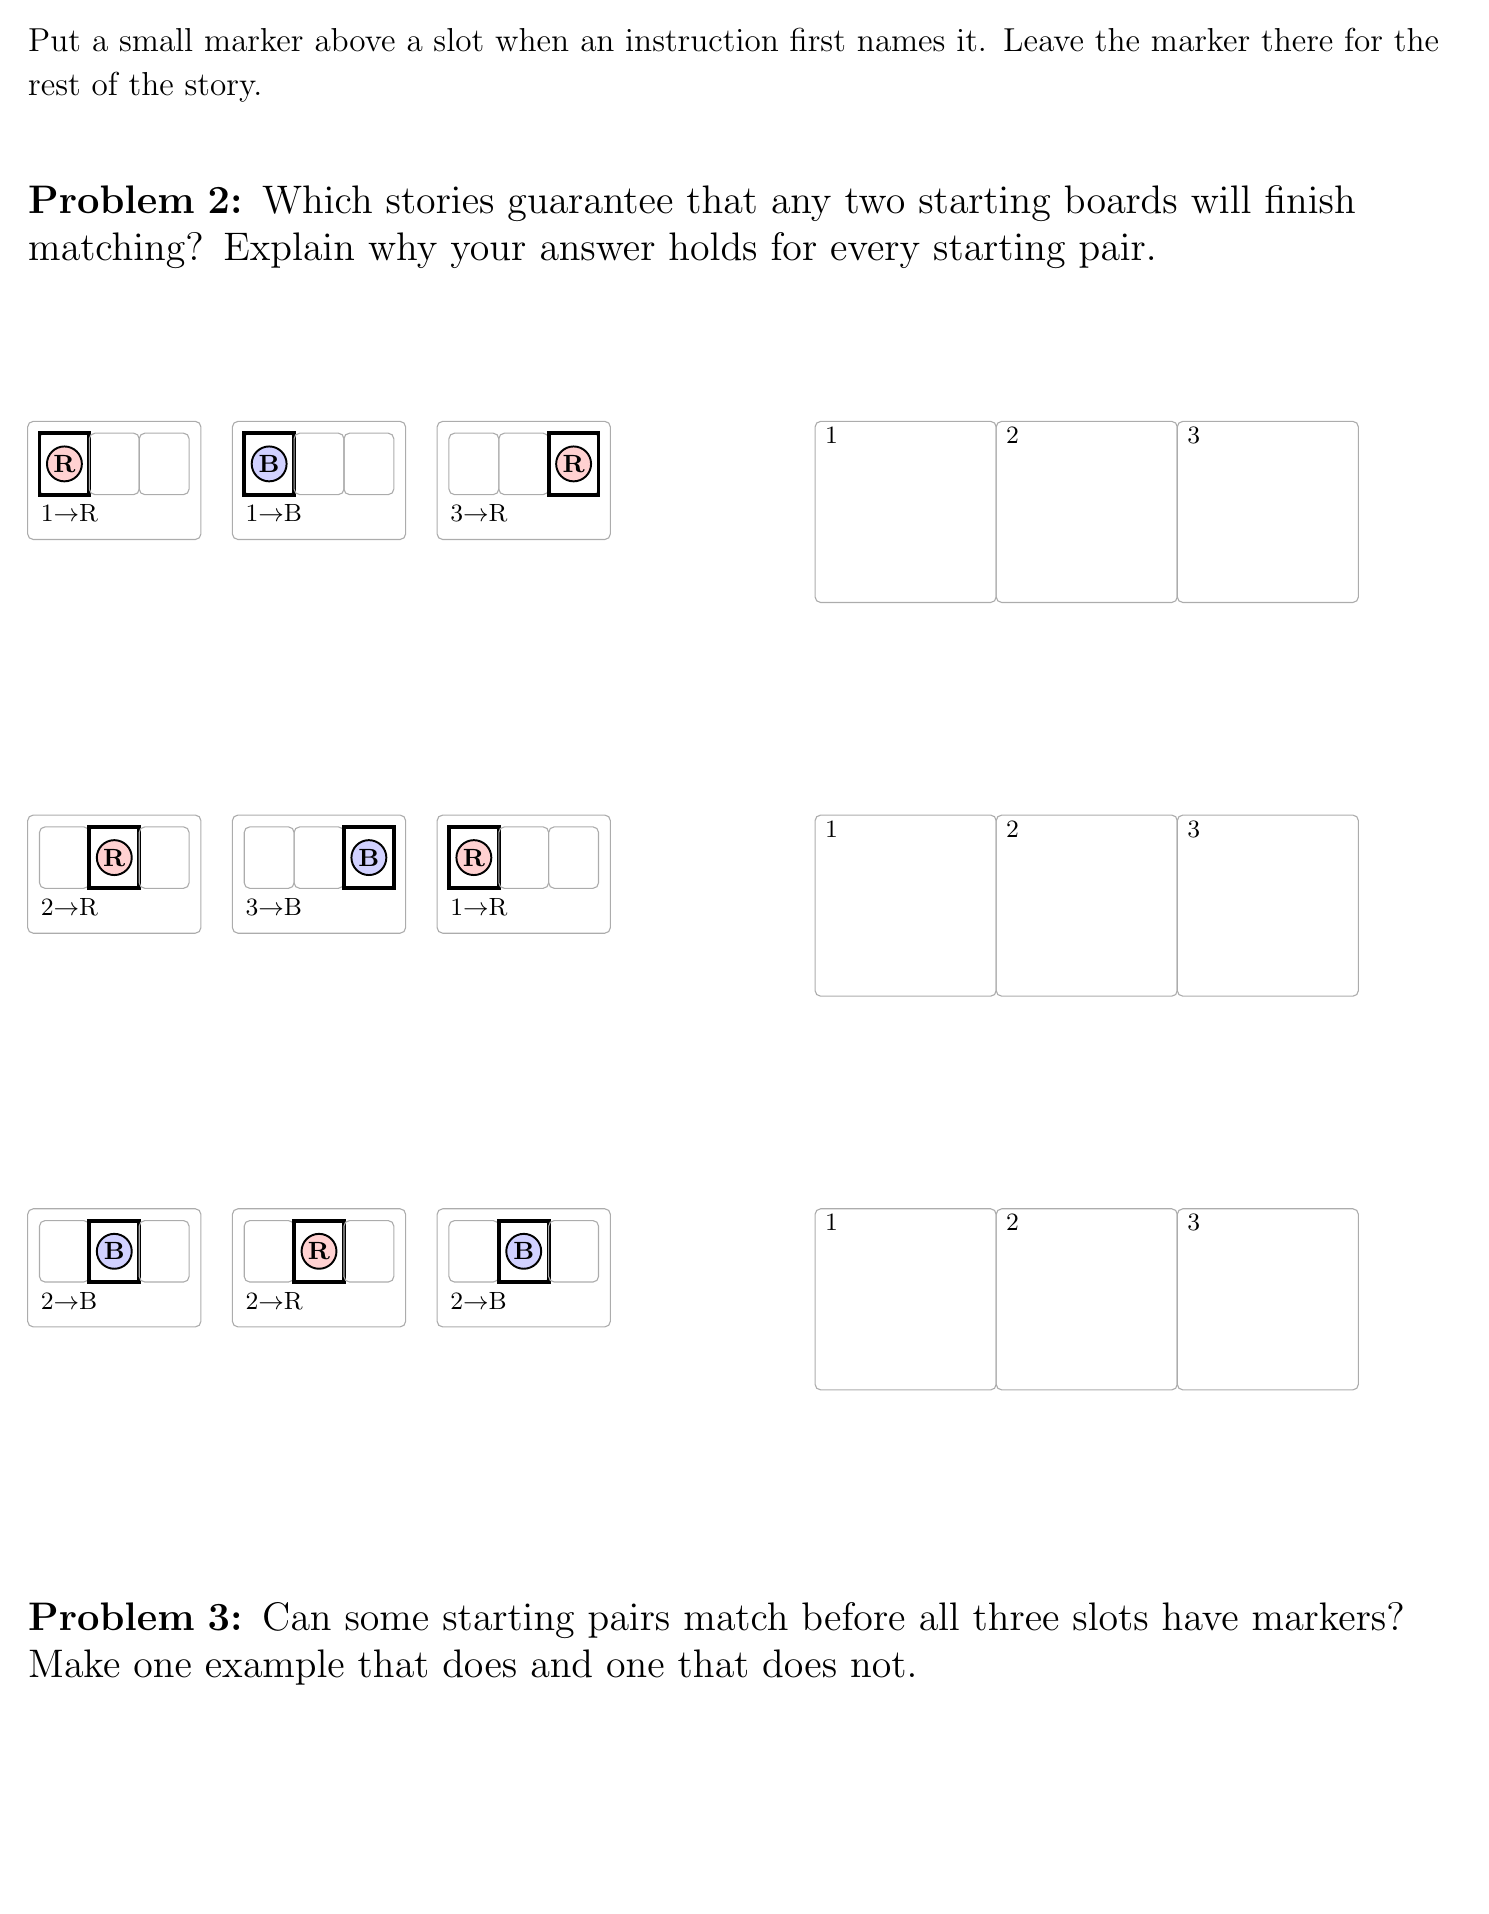
\begin{tikzpicture}[x=1cm,y=1cm]\path[use as bounding box] (0,0) rectangle (18.2,-23.6);
\node[anchor=north west,text width=18cm,inner sep=0pt,font=\fontsize{13}{16}\selectfont] at (0,0) {Put a small marker above a slot when an instruction first names it. Leave the marker there for the rest of the story.};
\node[anchor=north west,text width=18cm,inner sep=0pt,font=\fontsize{14}{17}\selectfont] at (0,-2) {\textbf{Problem 2:} Which stories guarantee that any two starting boards will finish matching? Explain why your answer holds for every starting pair.};
\draw[gray!65,rounded corners=2pt] (0.0,-5) rectangle (2.2,-6.5);
\draw[gray!65,rounded corners=2pt] (0.15,-5.15) rectangle (0.7833333333333334,-5.930000000000001);
\draw[line width=1.4pt] (0.15,-5.15) rectangle (0.7833333333333334,-5.93);
\draw[fill=red!18,line width=.7pt] (0.4666666666666667,-5.54) circle (0.22166666666666668);
\node[font=\bfseries\small] at (0.4666666666666667,-5.54) {R};
\draw[gray!65,rounded corners=2pt] (0.7833333333333334,-5.15) rectangle (1.416666666666667,-5.930000000000001);
\draw[gray!65,rounded corners=2pt] (1.4166666666666667,-5.15) rectangle (2.0500000000000003,-5.930000000000001);
\node[anchor=north west,text width=2.0cm,inner sep=0pt,font=\fontsize{9}{12}\selectfont] at (0.16,-6.05) {1$\to$R};
\draw[gray!65,rounded corners=2pt] (2.6,-5) rectangle (4.800000000000001,-6.5);
\draw[gray!65,rounded corners=2pt] (2.75,-5.15) rectangle (3.3833333333333333,-5.930000000000001);
\draw[line width=1.4pt] (2.75,-5.15) rectangle (3.3833333333333333,-5.93);
\draw[fill=blue!18,line width=.7pt] (3.066666666666667,-5.54) circle (0.22166666666666668);
\node[font=\bfseries\small] at (3.066666666666667,-5.54) {B};
\draw[gray!65,rounded corners=2pt] (3.3833333333333333,-5.15) rectangle (4.016666666666667,-5.930000000000001);
\draw[gray!65,rounded corners=2pt] (4.016666666666667,-5.15) rectangle (4.65,-5.930000000000001);
\node[anchor=north west,text width=2.0cm,inner sep=0pt,font=\fontsize{9}{12}\selectfont] at (2.7600000000000002,-6.05) {1$\to$B};
\draw[gray!65,rounded corners=2pt] (5.2,-5) rectangle (7.4,-6.5);
\draw[gray!65,rounded corners=2pt] (5.3500000000000005,-5.15) rectangle (5.983333333333334,-5.930000000000001);
\draw[gray!65,rounded corners=2pt] (5.983333333333334,-5.15) rectangle (6.616666666666668,-5.930000000000001);
\draw[gray!65,rounded corners=2pt] (6.616666666666667,-5.15) rectangle (7.250000000000001,-5.930000000000001);
\draw[line width=1.4pt] (6.616666666666667,-5.15) rectangle (7.250000000000001,-5.93);
\draw[fill=red!18,line width=.7pt] (6.933333333333334,-5.54) circle (0.22166666666666668);
\node[font=\bfseries\small] at (6.933333333333334,-5.54) {R};
\node[anchor=north west,text width=2.0cm,inner sep=0pt,font=\fontsize{9}{12}\selectfont] at (5.36,-6.05) {3$\to$R};
\draw[gray!65,rounded corners=2pt] (10.0,-5) rectangle (12.3,-7.3);
\node[anchor=north west,text width=0.6cm,inner sep=0pt,font=\fontsize{9}{12}\selectfont] at (10.12,-5.07) {1};
\draw[gray!65,rounded corners=2pt] (12.3,-5) rectangle (14.600000000000001,-7.3);
\node[anchor=north west,text width=0.6cm,inner sep=0pt,font=\fontsize{9}{12}\selectfont] at (12.42,-5.07) {2};
\draw[gray!65,rounded corners=2pt] (14.6,-5) rectangle (16.9,-7.3);
\node[anchor=north west,text width=0.6cm,inner sep=0pt,font=\fontsize{9}{12}\selectfont] at (14.719999999999999,-5.07) {3};
\draw[gray!65,rounded corners=2pt] (0.0,-10) rectangle (2.2,-11.5);
\draw[gray!65,rounded corners=2pt] (0.15,-10.15) rectangle (0.7833333333333334,-10.93);
\draw[gray!65,rounded corners=2pt] (0.7833333333333334,-10.15) rectangle (1.416666666666667,-10.93);
\draw[line width=1.4pt] (0.7833333333333334,-10.15) rectangle (1.416666666666667,-10.93);
\draw[fill=red!18,line width=.7pt] (1.1,-10.54) circle (0.22166666666666668);
\node[font=\bfseries\small] at (1.1,-10.54) {R};
\draw[gray!65,rounded corners=2pt] (1.4166666666666667,-10.15) rectangle (2.0500000000000003,-10.93);
\node[anchor=north west,text width=2.0cm,inner sep=0pt,font=\fontsize{9}{12}\selectfont] at (0.16,-11.05) {2$\to$R};
\draw[gray!65,rounded corners=2pt] (2.6,-10) rectangle (4.800000000000001,-11.5);
\draw[gray!65,rounded corners=2pt] (2.75,-10.15) rectangle (3.3833333333333333,-10.93);
\draw[gray!65,rounded corners=2pt] (3.3833333333333333,-10.15) rectangle (4.016666666666667,-10.93);
\draw[gray!65,rounded corners=2pt] (4.016666666666667,-10.15) rectangle (4.65,-10.93);
\draw[line width=1.4pt] (4.016666666666667,-10.15) rectangle (4.65,-10.93);
\draw[fill=blue!18,line width=.7pt] (4.333333333333333,-10.54) circle (0.22166666666666668);
\node[font=\bfseries\small] at (4.333333333333333,-10.54) {B};
\node[anchor=north west,text width=2.0cm,inner sep=0pt,font=\fontsize{9}{12}\selectfont] at (2.7600000000000002,-11.05) {3$\to$B};
\draw[gray!65,rounded corners=2pt] (5.2,-10) rectangle (7.4,-11.5);
\draw[gray!65,rounded corners=2pt] (5.3500000000000005,-10.15) rectangle (5.983333333333334,-10.93);
\draw[line width=1.4pt] (5.3500000000000005,-10.15) rectangle (5.983333333333334,-10.93);
\draw[fill=red!18,line width=.7pt] (5.666666666666667,-10.54) circle (0.22166666666666668);
\node[font=\bfseries\small] at (5.666666666666667,-10.54) {R};
\draw[gray!65,rounded corners=2pt] (5.983333333333334,-10.15) rectangle (6.616666666666668,-10.93);
\draw[gray!65,rounded corners=2pt] (6.616666666666667,-10.15) rectangle (7.250000000000001,-10.93);
\node[anchor=north west,text width=2.0cm,inner sep=0pt,font=\fontsize{9}{12}\selectfont] at (5.36,-11.05) {1$\to$R};
\draw[gray!65,rounded corners=2pt] (10.0,-10) rectangle (12.3,-12.3);
\node[anchor=north west,text width=0.6cm,inner sep=0pt,font=\fontsize{9}{12}\selectfont] at (10.12,-10.07) {1};
\draw[gray!65,rounded corners=2pt] (12.3,-10) rectangle (14.600000000000001,-12.3);
\node[anchor=north west,text width=0.6cm,inner sep=0pt,font=\fontsize{9}{12}\selectfont] at (12.42,-10.07) {2};
\draw[gray!65,rounded corners=2pt] (14.6,-10) rectangle (16.9,-12.3);
\node[anchor=north west,text width=0.6cm,inner sep=0pt,font=\fontsize{9}{12}\selectfont] at (14.719999999999999,-10.07) {3};
\draw[gray!65,rounded corners=2pt] (0.0,-15) rectangle (2.2,-16.5);
\draw[gray!65,rounded corners=2pt] (0.15,-15.15) rectangle (0.7833333333333334,-15.93);
\draw[gray!65,rounded corners=2pt] (0.7833333333333334,-15.15) rectangle (1.416666666666667,-15.93);
\draw[line width=1.4pt] (0.7833333333333334,-15.15) rectangle (1.416666666666667,-15.93);
\draw[fill=blue!18,line width=.7pt] (1.1,-15.54) circle (0.22166666666666668);
\node[font=\bfseries\small] at (1.1,-15.54) {B};
\draw[gray!65,rounded corners=2pt] (1.4166666666666667,-15.15) rectangle (2.0500000000000003,-15.93);
\node[anchor=north west,text width=2.0cm,inner sep=0pt,font=\fontsize{9}{12}\selectfont] at (0.16,-16.05) {2$\to$B};
\draw[gray!65,rounded corners=2pt] (2.6,-15) rectangle (4.800000000000001,-16.5);
\draw[gray!65,rounded corners=2pt] (2.75,-15.15) rectangle (3.3833333333333333,-15.93);
\draw[gray!65,rounded corners=2pt] (3.3833333333333333,-15.15) rectangle (4.016666666666667,-15.93);
\draw[line width=1.4pt] (3.3833333333333333,-15.15) rectangle (4.016666666666667,-15.93);
\draw[fill=red!18,line width=.7pt] (3.7,-15.54) circle (0.22166666666666668);
\node[font=\bfseries\small] at (3.7,-15.54) {R};
\draw[gray!65,rounded corners=2pt] (4.016666666666667,-15.15) rectangle (4.65,-15.93);
\node[anchor=north west,text width=2.0cm,inner sep=0pt,font=\fontsize{9}{12}\selectfont] at (2.7600000000000002,-16.05) {2$\to$R};
\draw[gray!65,rounded corners=2pt] (5.2,-15) rectangle (7.4,-16.5);
\draw[gray!65,rounded corners=2pt] (5.3500000000000005,-15.15) rectangle (5.983333333333334,-15.93);
\draw[gray!65,rounded corners=2pt] (5.983333333333334,-15.15) rectangle (6.616666666666668,-15.93);
\draw[line width=1.4pt] (5.983333333333334,-15.15) rectangle (6.616666666666668,-15.93);
\draw[fill=blue!18,line width=.7pt] (6.300000000000001,-15.54) circle (0.22166666666666668);
\node[font=\bfseries\small] at (6.300000000000001,-15.54) {B};
\draw[gray!65,rounded corners=2pt] (6.616666666666667,-15.15) rectangle (7.250000000000001,-15.93);
\node[anchor=north west,text width=2.0cm,inner sep=0pt,font=\fontsize{9}{12}\selectfont] at (5.36,-16.05) {2$\to$B};
\draw[gray!65,rounded corners=2pt] (10.0,-15) rectangle (12.3,-17.3);
\node[anchor=north west,text width=0.6cm,inner sep=0pt,font=\fontsize{9}{12}\selectfont] at (10.12,-15.07) {1};
\draw[gray!65,rounded corners=2pt] (12.3,-15) rectangle (14.600000000000001,-17.3);
\node[anchor=north west,text width=0.6cm,inner sep=0pt,font=\fontsize{9}{12}\selectfont] at (12.42,-15.07) {2};
\draw[gray!65,rounded corners=2pt] (14.6,-15) rectangle (16.9,-17.3);
\node[anchor=north west,text width=0.6cm,inner sep=0pt,font=\fontsize{9}{12}\selectfont] at (14.719999999999999,-15.07) {3};
\node[anchor=north west,text width=18cm,inner sep=0pt,font=\fontsize{14}{17}\selectfont] at (0,-20) {\textbf{Problem 3:} Can some starting pairs match before all three slots have markers? Make one example that does and one that does not.};
\end{tikzpicture}
\newpage
\noindent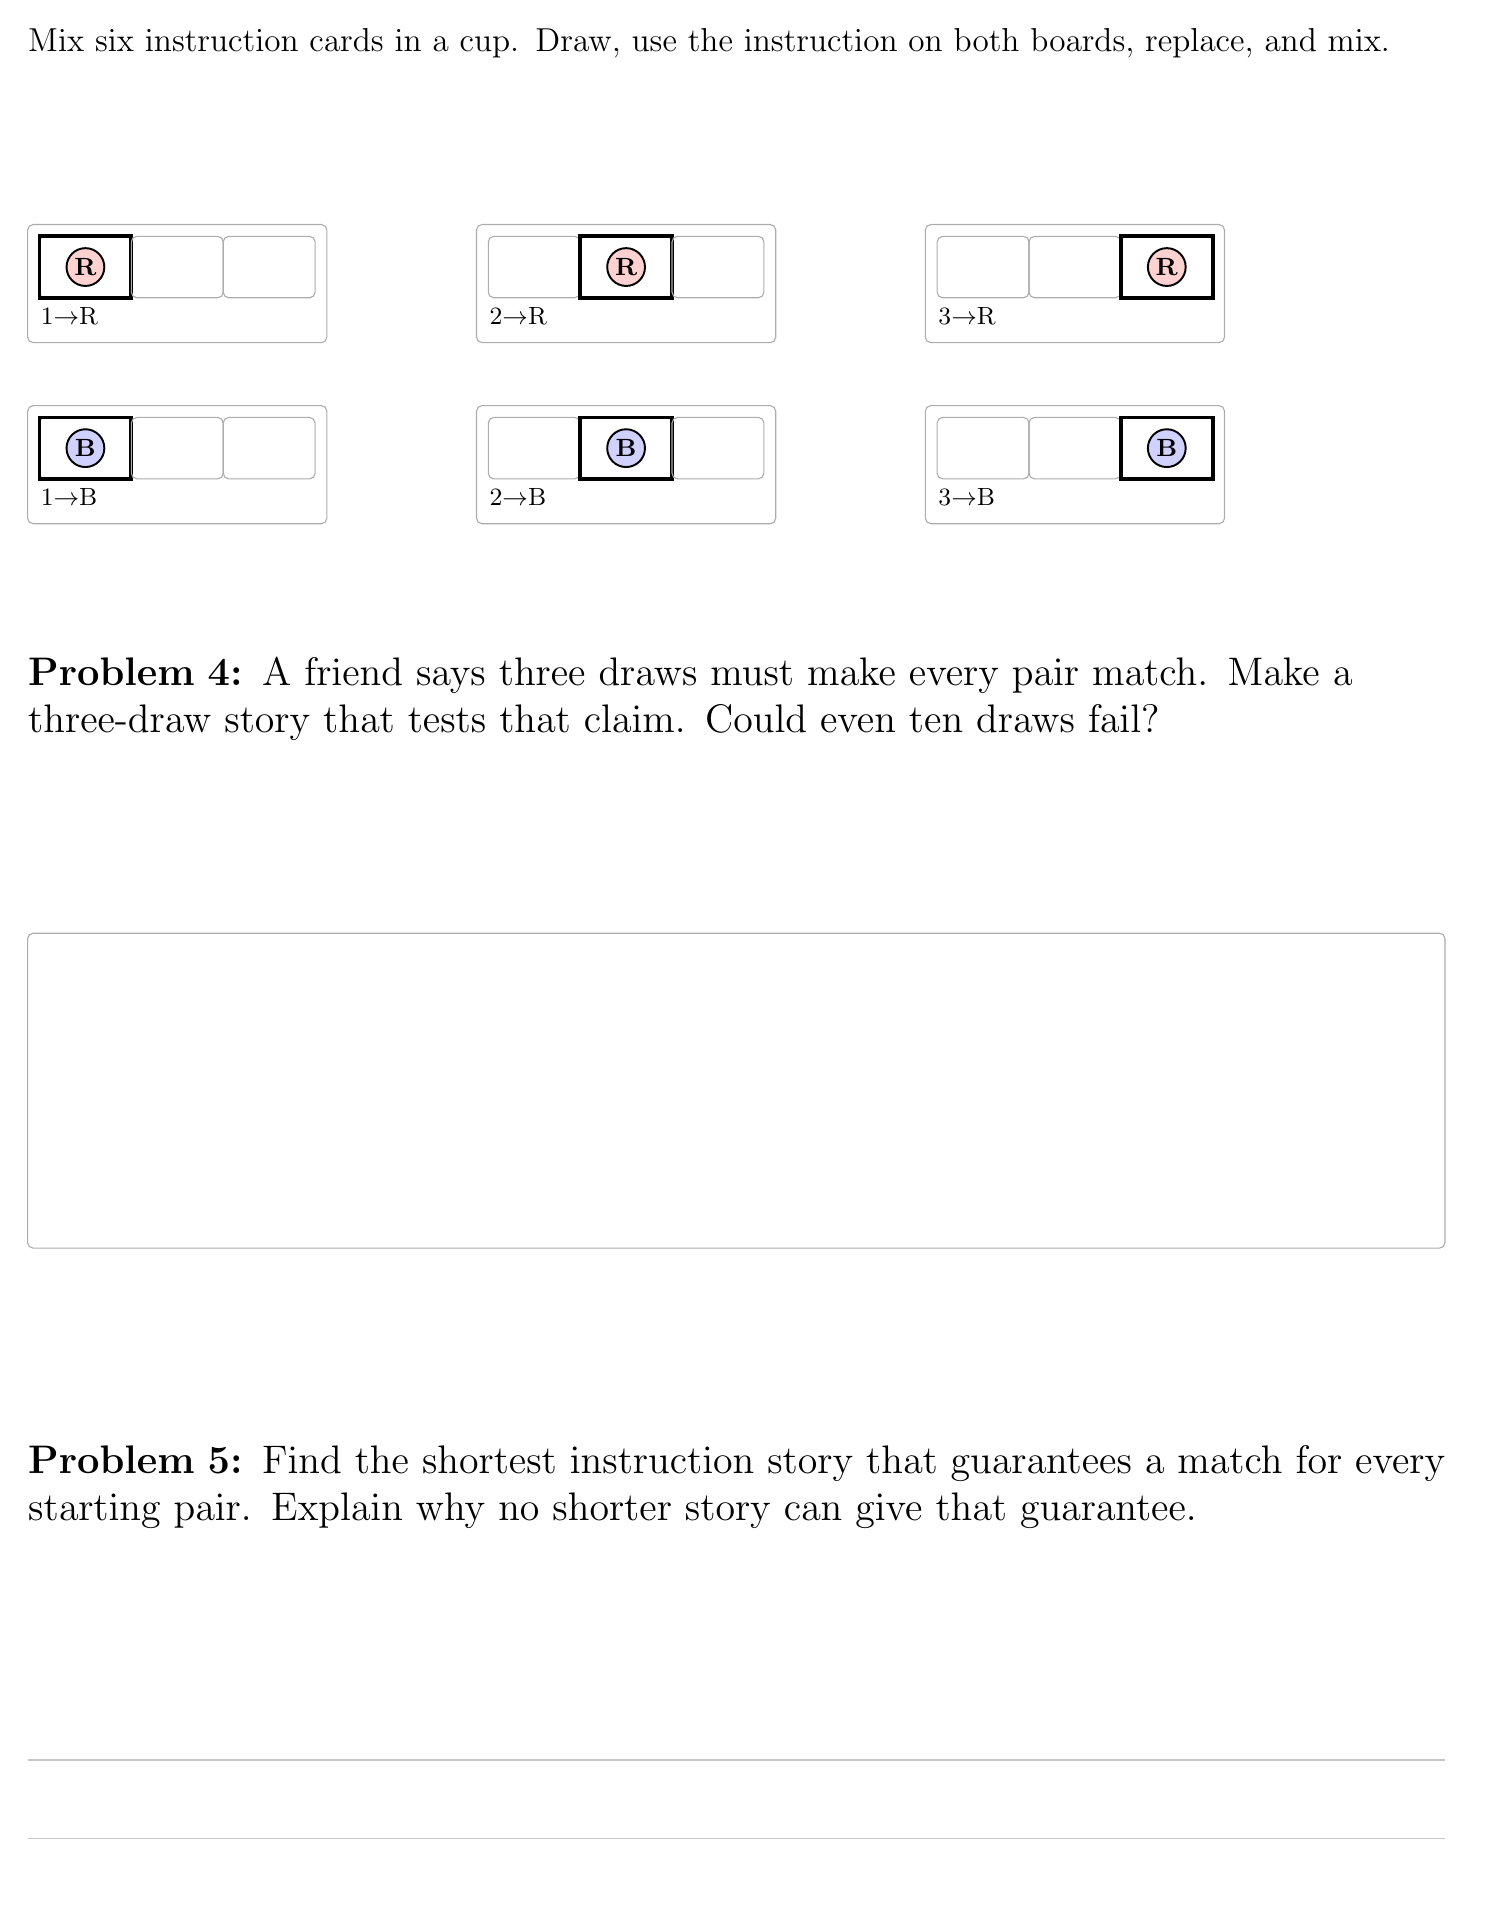
\begin{tikzpicture}[x=1cm,y=1cm]\path[use as bounding box] (0,0) rectangle (18.2,-23.6);
\node[anchor=north west,text width=18cm,inner sep=0pt,font=\fontsize{13}{16}\selectfont] at (0,0) {Mix six instruction cards in a cup. Draw, use the instruction on both boards, replace, and mix.};
\draw[gray!65,rounded corners=2pt] (0.0,-2.5) rectangle (3.8,-4.0);
\draw[gray!65,rounded corners=2pt] (0.15,-2.65) rectangle (1.3166666666666667,-3.4299999999999997);
\draw[line width=1.4pt] (0.15,-2.65) rectangle (1.3166666666666667,-3.43);
\draw[fill=red!18,line width=.7pt] (0.7333333333333334,-3.04) circle (0.24);
\node[font=\bfseries\small] at (0.7333333333333334,-3.04) {R};
\draw[gray!65,rounded corners=2pt] (1.3166666666666667,-2.65) rectangle (2.4833333333333334,-3.4299999999999997);
\draw[gray!65,rounded corners=2pt] (2.4833333333333334,-2.65) rectangle (3.6500000000000004,-3.4299999999999997);
\node[anchor=north west,text width=3.5999999999999996cm,inner sep=0pt,font=\fontsize{9}{12}\selectfont] at (0.16,-3.55) {1$\to$R};
\draw[gray!65,rounded corners=2pt] (5.7,-2.5) rectangle (9.5,-4.0);
\draw[gray!65,rounded corners=2pt] (5.8500000000000005,-2.65) rectangle (7.0166666666666675,-3.4299999999999997);
\draw[gray!65,rounded corners=2pt] (7.0166666666666675,-2.65) rectangle (8.183333333333334,-3.4299999999999997);
\draw[line width=1.4pt] (7.0166666666666675,-2.65) rectangle (8.183333333333334,-3.43);
\draw[fill=red!18,line width=.7pt] (7.6000000000000005,-3.04) circle (0.24);
\node[font=\bfseries\small] at (7.6000000000000005,-3.04) {R};
\draw[gray!65,rounded corners=2pt] (8.183333333333334,-2.65) rectangle (9.35,-3.4299999999999997);
\node[anchor=north west,text width=3.5999999999999996cm,inner sep=0pt,font=\fontsize{9}{12}\selectfont] at (5.86,-3.55) {2$\to$R};
\draw[gray!65,rounded corners=2pt] (11.4,-2.5) rectangle (15.2,-4.0);
\draw[gray!65,rounded corners=2pt] (11.55,-2.65) rectangle (12.716666666666667,-3.4299999999999997);
\draw[gray!65,rounded corners=2pt] (12.716666666666667,-2.65) rectangle (13.883333333333333,-3.4299999999999997);
\draw[gray!65,rounded corners=2pt] (13.883333333333335,-2.65) rectangle (15.05,-3.4299999999999997);
\draw[line width=1.4pt] (13.883333333333335,-2.65) rectangle (15.05,-3.43);
\draw[fill=red!18,line width=.7pt] (14.466666666666669,-3.04) circle (0.24);
\node[font=\bfseries\small] at (14.466666666666669,-3.04) {R};
\node[anchor=north west,text width=3.5999999999999996cm,inner sep=0pt,font=\fontsize{9}{12}\selectfont] at (11.56,-3.55) {3$\to$R};
\draw[gray!65,rounded corners=2pt] (0.0,-4.8) rectangle (3.8,-6.3);
\draw[gray!65,rounded corners=2pt] (0.15,-4.95) rectangle (1.3166666666666667,-5.73);
\draw[line width=1.4pt] (0.15,-4.95) rectangle (1.3166666666666667,-5.7299999999999995);
\draw[fill=blue!18,line width=.7pt] (0.7333333333333334,-5.34) circle (0.24);
\node[font=\bfseries\small] at (0.7333333333333334,-5.34) {B};
\draw[gray!65,rounded corners=2pt] (1.3166666666666667,-4.95) rectangle (2.4833333333333334,-5.73);
\draw[gray!65,rounded corners=2pt] (2.4833333333333334,-4.95) rectangle (3.6500000000000004,-5.73);
\node[anchor=north west,text width=3.5999999999999996cm,inner sep=0pt,font=\fontsize{9}{12}\selectfont] at (0.16,-5.85) {1$\to$B};
\draw[gray!65,rounded corners=2pt] (5.7,-4.8) rectangle (9.5,-6.3);
\draw[gray!65,rounded corners=2pt] (5.8500000000000005,-4.95) rectangle (7.0166666666666675,-5.73);
\draw[gray!65,rounded corners=2pt] (7.0166666666666675,-4.95) rectangle (8.183333333333334,-5.73);
\draw[line width=1.4pt] (7.0166666666666675,-4.95) rectangle (8.183333333333334,-5.7299999999999995);
\draw[fill=blue!18,line width=.7pt] (7.6000000000000005,-5.34) circle (0.24);
\node[font=\bfseries\small] at (7.6000000000000005,-5.34) {B};
\draw[gray!65,rounded corners=2pt] (8.183333333333334,-4.95) rectangle (9.35,-5.73);
\node[anchor=north west,text width=3.5999999999999996cm,inner sep=0pt,font=\fontsize{9}{12}\selectfont] at (5.86,-5.85) {2$\to$B};
\draw[gray!65,rounded corners=2pt] (11.4,-4.8) rectangle (15.2,-6.3);
\draw[gray!65,rounded corners=2pt] (11.55,-4.95) rectangle (12.716666666666667,-5.73);
\draw[gray!65,rounded corners=2pt] (12.716666666666667,-4.95) rectangle (13.883333333333333,-5.73);
\draw[gray!65,rounded corners=2pt] (13.883333333333335,-4.95) rectangle (15.05,-5.73);
\draw[line width=1.4pt] (13.883333333333335,-4.95) rectangle (15.05,-5.7299999999999995);
\draw[fill=blue!18,line width=.7pt] (14.466666666666669,-5.34) circle (0.24);
\node[font=\bfseries\small] at (14.466666666666669,-5.34) {B};
\node[anchor=north west,text width=3.5999999999999996cm,inner sep=0pt,font=\fontsize{9}{12}\selectfont] at (11.56,-5.85) {3$\to$B};
\node[anchor=north west,text width=18cm,inner sep=0pt,font=\fontsize{14}{17}\selectfont] at (0,-8) {\textbf{Problem 4:} A friend says three draws must make every pair match. Make a three-draw story that tests that claim. Could even ten draws fail?};
\draw[gray!65,rounded corners=2pt] (0,-11.5) rectangle (18,-15.5);
\node[anchor=north west,text width=18cm,inner sep=0pt,font=\fontsize{14}{17}\selectfont] at (0,-18) {\textbf{Problem 5:} Find the shortest instruction story that guarantees a match for every starting pair. Explain why no shorter story can give that guarantee.};
\draw[gray!45] (0,-22) -- (18,-22);
\draw[gray!45] (0,-23) -- (18,-23);
\end{tikzpicture}
\newpage
\noindent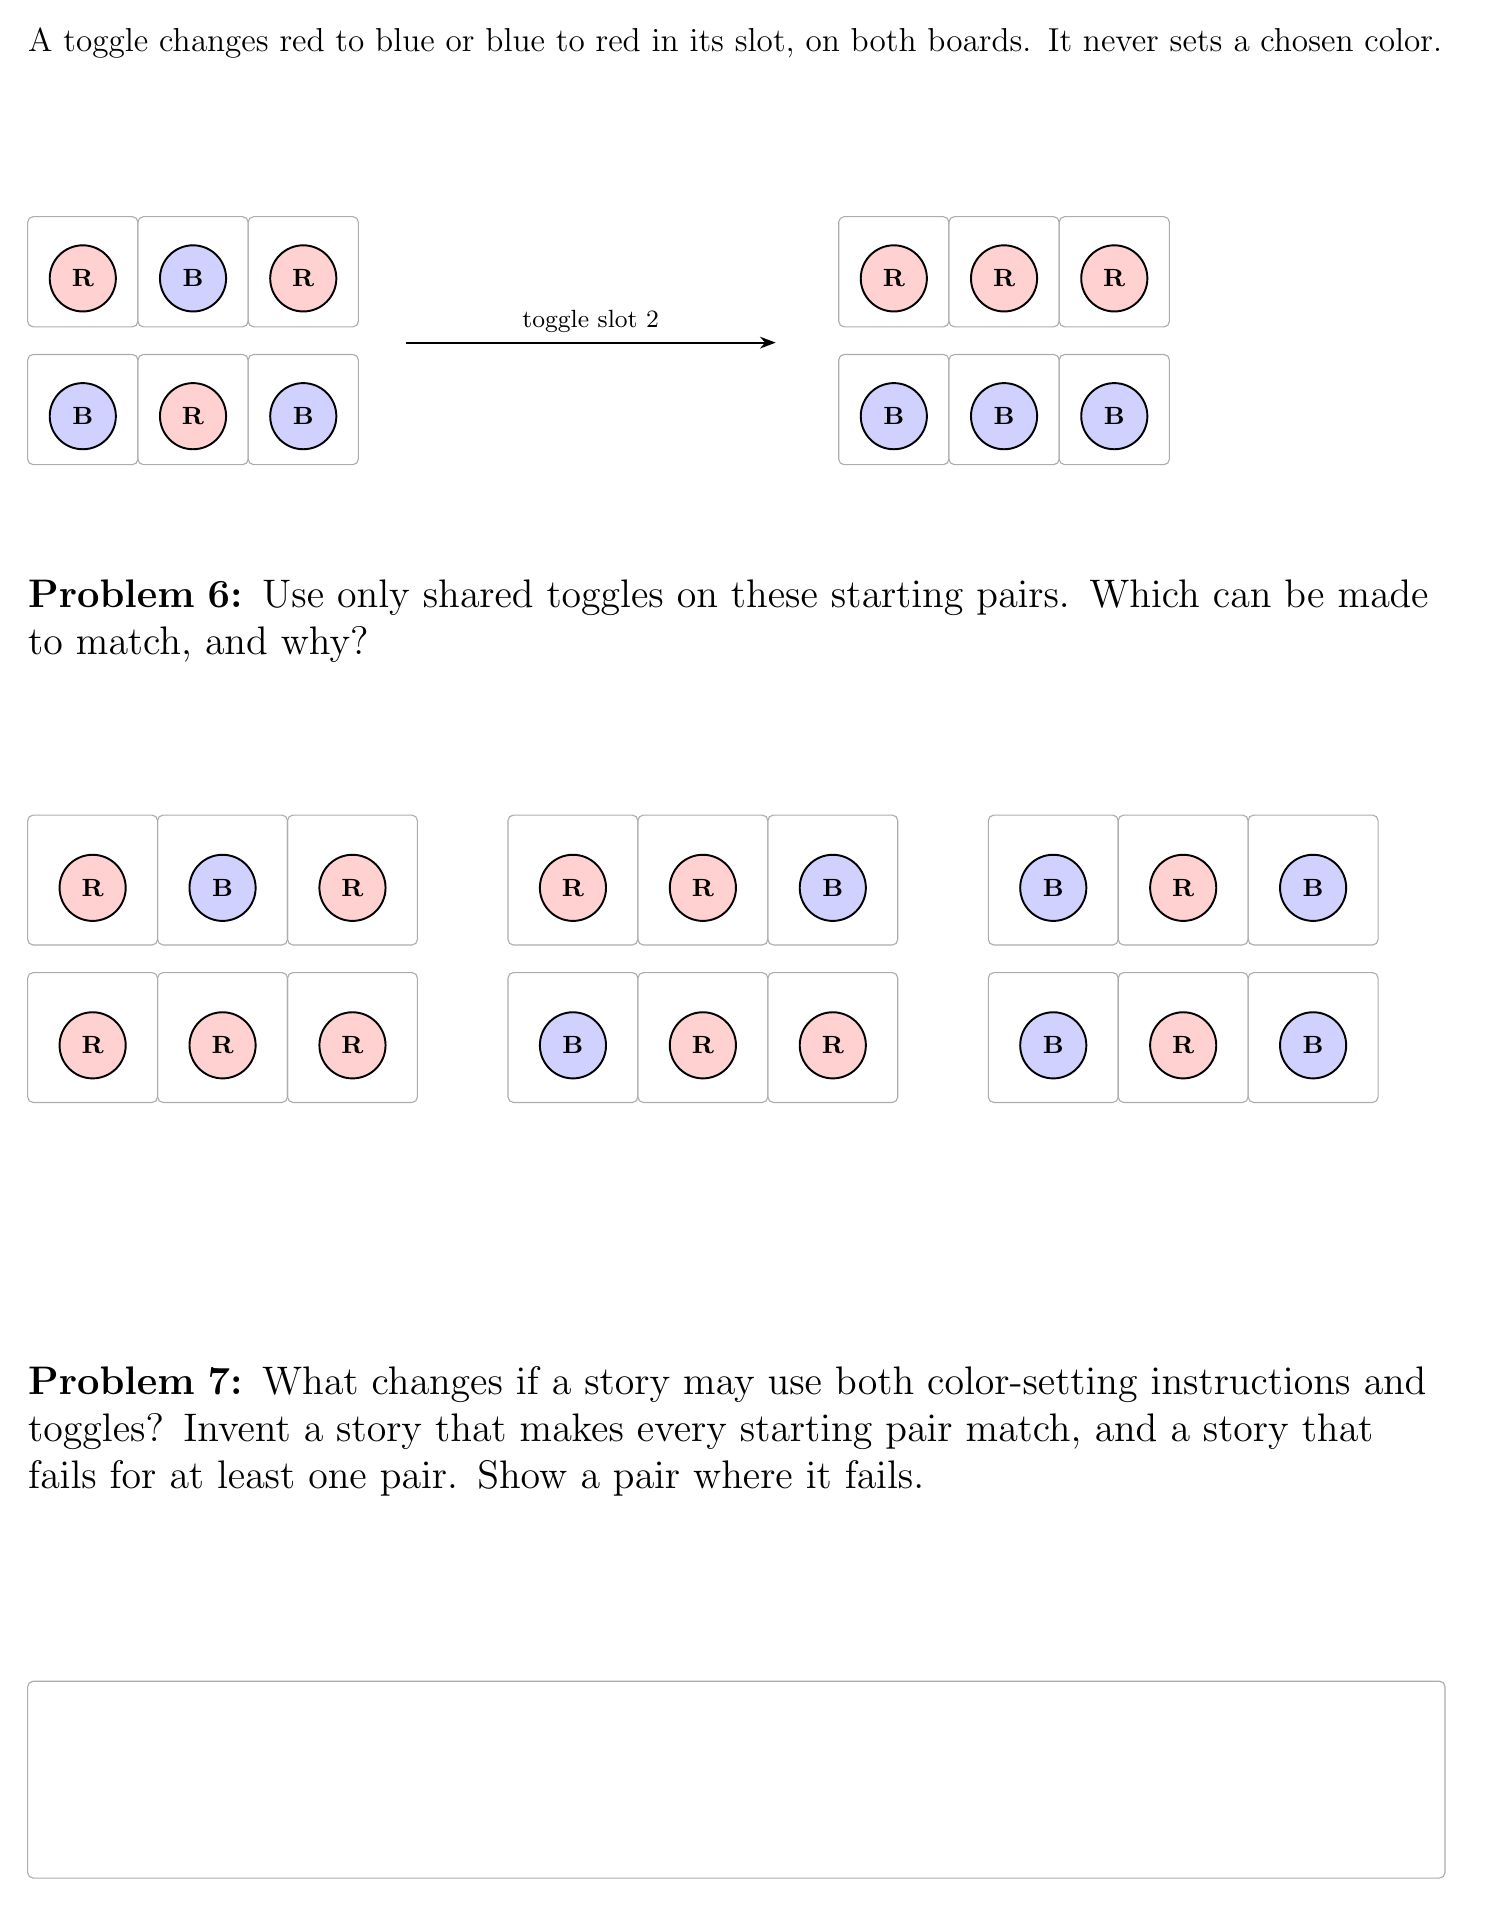
\begin{tikzpicture}[x=1cm,y=1cm]\path[use as bounding box] (0,0) rectangle (18.2,-23.6);
\node[anchor=north west,text width=18cm,inner sep=0pt,font=\fontsize{13}{16}\selectfont] at (0,0) {A toggle changes red to blue or blue to red in its slot, on both boards. It never sets a chosen color.};
\draw[gray!65,rounded corners=2pt] (0.0,-2.4) rectangle (1.4,-3.8);
\draw[fill=red!18,line width=.7pt] (0.7,-3.184) circle (0.42);
\node[font=\bfseries\small] at (0.7,-3.184) {R};
\draw[gray!65,rounded corners=2pt] (1.4,-2.4) rectangle (2.8,-3.8);
\draw[fill=blue!18,line width=.7pt] (2.0999999999999996,-3.184) circle (0.42);
\node[font=\bfseries\small] at (2.0999999999999996,-3.184) {B};
\draw[gray!65,rounded corners=2pt] (2.8,-2.4) rectangle (4.199999999999999,-3.8);
\draw[fill=red!18,line width=.7pt] (3.5,-3.184) circle (0.42);
\node[font=\bfseries\small] at (3.5,-3.184) {R};
\draw[gray!65,rounded corners=2pt] (0.0,-4.1499999999999995) rectangle (1.4,-5.549999999999999);
\draw[fill=blue!18,line width=.7pt] (0.7,-4.933999999999999) circle (0.42);
\node[font=\bfseries\small] at (0.7,-4.933999999999999) {B};
\draw[gray!65,rounded corners=2pt] (1.4,-4.1499999999999995) rectangle (2.8,-5.549999999999999);
\draw[fill=red!18,line width=.7pt] (2.0999999999999996,-4.933999999999999) circle (0.42);
\node[font=\bfseries\small] at (2.0999999999999996,-4.933999999999999) {R};
\draw[gray!65,rounded corners=2pt] (2.8,-4.1499999999999995) rectangle (4.199999999999999,-5.549999999999999);
\draw[fill=blue!18,line width=.7pt] (3.5,-4.933999999999999) circle (0.42);
\node[font=\bfseries\small] at (3.5,-4.933999999999999) {B};
\draw[-{Stealth[length=2mm]},line width=.8pt] (4.8,-4) -- (9.5,-4) node[midway,above,font=\small] {toggle slot 2};
\draw[gray!65,rounded corners=2pt] (10.3,-2.4) rectangle (11.700000000000001,-3.8);
\draw[fill=red!18,line width=.7pt] (11.0,-3.184) circle (0.42);
\node[font=\bfseries\small] at (11.0,-3.184) {R};
\draw[gray!65,rounded corners=2pt] (11.700000000000001,-2.4) rectangle (13.100000000000001,-3.8);
\draw[fill=red!18,line width=.7pt] (12.4,-3.184) circle (0.42);
\node[font=\bfseries\small] at (12.4,-3.184) {R};
\draw[gray!65,rounded corners=2pt] (13.100000000000001,-2.4) rectangle (14.500000000000002,-3.8);
\draw[fill=red!18,line width=.7pt] (13.8,-3.184) circle (0.42);
\node[font=\bfseries\small] at (13.8,-3.184) {R};
\draw[gray!65,rounded corners=2pt] (10.3,-4.1499999999999995) rectangle (11.700000000000001,-5.549999999999999);
\draw[fill=blue!18,line width=.7pt] (11.0,-4.933999999999999) circle (0.42);
\node[font=\bfseries\small] at (11.0,-4.933999999999999) {B};
\draw[gray!65,rounded corners=2pt] (11.700000000000001,-4.1499999999999995) rectangle (13.100000000000001,-5.549999999999999);
\draw[fill=blue!18,line width=.7pt] (12.4,-4.933999999999999) circle (0.42);
\node[font=\bfseries\small] at (12.4,-4.933999999999999) {B};
\draw[gray!65,rounded corners=2pt] (13.100000000000001,-4.1499999999999995) rectangle (14.500000000000002,-5.549999999999999);
\draw[fill=blue!18,line width=.7pt] (13.8,-4.933999999999999) circle (0.42);
\node[font=\bfseries\small] at (13.8,-4.933999999999999) {B};
\node[anchor=north west,text width=18cm,inner sep=0pt,font=\fontsize{14}{17}\selectfont] at (0,-7) {\textbf{Problem 6:} Use only shared toggles on these starting pairs. Which can be made to match, and why?};
\draw[gray!65,rounded corners=2pt] (0.0,-10) rectangle (1.65,-11.65);
\draw[fill=red!18,line width=.7pt] (0.825,-10.924) circle (0.42);
\node[font=\bfseries\small] at (0.825,-10.924) {R};
\draw[gray!65,rounded corners=2pt] (1.65,-10) rectangle (3.3,-11.65);
\draw[fill=blue!18,line width=.7pt] (2.4749999999999996,-10.924) circle (0.42);
\node[font=\bfseries\small] at (2.4749999999999996,-10.924) {B};
\draw[gray!65,rounded corners=2pt] (3.3,-10) rectangle (4.949999999999999,-11.65);
\draw[fill=red!18,line width=.7pt] (4.125,-10.924) circle (0.42);
\node[font=\bfseries\small] at (4.125,-10.924) {R};
\draw[gray!65,rounded corners=2pt] (0.0,-12.0) rectangle (1.65,-13.65);
\draw[fill=red!18,line width=.7pt] (0.825,-12.924) circle (0.42);
\node[font=\bfseries\small] at (0.825,-12.924) {R};
\draw[gray!65,rounded corners=2pt] (1.65,-12.0) rectangle (3.3,-13.65);
\draw[fill=red!18,line width=.7pt] (2.4749999999999996,-12.924) circle (0.42);
\node[font=\bfseries\small] at (2.4749999999999996,-12.924) {R};
\draw[gray!65,rounded corners=2pt] (3.3,-12.0) rectangle (4.949999999999999,-13.65);
\draw[fill=red!18,line width=.7pt] (4.125,-12.924) circle (0.42);
\node[font=\bfseries\small] at (4.125,-12.924) {R};
\draw[gray!65,rounded corners=2pt] (6.1,-10) rectangle (7.75,-11.65);
\draw[fill=red!18,line width=.7pt] (6.925,-10.924) circle (0.42);
\node[font=\bfseries\small] at (6.925,-10.924) {R};
\draw[gray!65,rounded corners=2pt] (7.75,-10) rectangle (9.4,-11.65);
\draw[fill=red!18,line width=.7pt] (8.575,-10.924) circle (0.42);
\node[font=\bfseries\small] at (8.575,-10.924) {R};
\draw[gray!65,rounded corners=2pt] (9.399999999999999,-10) rectangle (11.049999999999999,-11.65);
\draw[fill=blue!18,line width=.7pt] (10.225,-10.924) circle (0.42);
\node[font=\bfseries\small] at (10.225,-10.924) {B};
\draw[gray!65,rounded corners=2pt] (6.1,-12.0) rectangle (7.75,-13.65);
\draw[fill=blue!18,line width=.7pt] (6.925,-12.924) circle (0.42);
\node[font=\bfseries\small] at (6.925,-12.924) {B};
\draw[gray!65,rounded corners=2pt] (7.75,-12.0) rectangle (9.4,-13.65);
\draw[fill=red!18,line width=.7pt] (8.575,-12.924) circle (0.42);
\node[font=\bfseries\small] at (8.575,-12.924) {R};
\draw[gray!65,rounded corners=2pt] (9.399999999999999,-12.0) rectangle (11.049999999999999,-13.65);
\draw[fill=red!18,line width=.7pt] (10.225,-12.924) circle (0.42);
\node[font=\bfseries\small] at (10.225,-12.924) {R};
\draw[gray!65,rounded corners=2pt] (12.2,-10) rectangle (13.85,-11.65);
\draw[fill=blue!18,line width=.7pt] (13.024999999999999,-10.924) circle (0.42);
\node[font=\bfseries\small] at (13.024999999999999,-10.924) {B};
\draw[gray!65,rounded corners=2pt] (13.85,-10) rectangle (15.5,-11.65);
\draw[fill=red!18,line width=.7pt] (14.674999999999999,-10.924) circle (0.42);
\node[font=\bfseries\small] at (14.674999999999999,-10.924) {R};
\draw[gray!65,rounded corners=2pt] (15.5,-10) rectangle (17.15,-11.65);
\draw[fill=blue!18,line width=.7pt] (16.325,-10.924) circle (0.42);
\node[font=\bfseries\small] at (16.325,-10.924) {B};
\draw[gray!65,rounded corners=2pt] (12.2,-12.0) rectangle (13.85,-13.65);
\draw[fill=blue!18,line width=.7pt] (13.024999999999999,-12.924) circle (0.42);
\node[font=\bfseries\small] at (13.024999999999999,-12.924) {B};
\draw[gray!65,rounded corners=2pt] (13.85,-12.0) rectangle (15.5,-13.65);
\draw[fill=red!18,line width=.7pt] (14.674999999999999,-12.924) circle (0.42);
\node[font=\bfseries\small] at (14.674999999999999,-12.924) {R};
\draw[gray!65,rounded corners=2pt] (15.5,-12.0) rectangle (17.15,-13.65);
\draw[fill=blue!18,line width=.7pt] (16.325,-12.924) circle (0.42);
\node[font=\bfseries\small] at (16.325,-12.924) {B};
\node[anchor=north west,text width=18cm,inner sep=0pt,font=\fontsize{14}{17}\selectfont] at (0,-17) {\textbf{Problem 7:} What changes if a story may use both color-setting instructions and toggles? Invent a story that makes every starting pair match, and a story that fails for at least one pair. Show a pair where it fails.};
\draw[gray!65,rounded corners=2pt] (0,-21) rectangle (18,-23.5);
\end{tikzpicture}
\end{document}
